% IEEE conference paper (IEEEtran, from the official template conference_101719.tex).
% Build on Overleaf (pdfLaTeX + BibTeX) or locally: latexmk -pdf main.tex
%
% Results are pulled in automatically once these files exist (copy them from the run):
%   cp runs/main/results_table.tex          paper/results/
%   cp runs/main/figures/test_Biogas.pdf    paper/results/
% Everything still to be filled from the run is printed in red by \tbd{...}.
% For a double-blind review version set \anontrue below.

\documentclass[conference]{IEEEtran}
\IEEEoverridecommandlockouts
\usepackage{cite}
\usepackage{amsmath,amssymb,amsfonts}
\usepackage{graphicx}
\usepackage{textcomp}
\usepackage{xcolor}
\usepackage{booktabs}
\usepackage{tikz}
\usetikzlibrary{positioning,arrows.meta,calc}
\usepackage[hidelinks]{hyperref}

\newcommand{\tbd}[1]{\textcolor{red}{[#1]}}
\newif\ifanon
\anonfalse % \anontrue for the review copy

\begin{document}

\title{Recurrent Neural Networks versus Lag-Feature Feed-Forward Networks for Daily Biogas Prediction at a Full-Scale Anaerobic Co-Digester}

\ifanon
\author{\IEEEauthorblockN{Anonymous Authors}\IEEEauthorblockA{Paper under double-blind review}}
\else
\author{
\IEEEauthorblockN{Roshan Jeyaruban R}
\IEEEauthorblockA{\textit{Dept. of Computer Science and Engineering (AI)}\\
\textit{Sathyabama Institute of Science and Technology}\\
Chennai, India\\
\tbd{email}}
\and
\IEEEauthorblockN{Akash Kumar K}
\IEEEauthorblockA{\textit{Dept. of Computer Science and Engineering (AI)}\\
\textit{Sathyabama Institute of Science and Technology}\\
Chennai, India\\
\tbd{email}}
\and
\IEEEauthorblockN{Dr.\ Shanthi Thangam M}
\IEEEauthorblockA{\textit{Dept. of Computer Science and Engineering}\\
\textit{Sathyabama Institute of Science and Technology}\\
Chennai, India\\
\tbd{email}}
}
\fi

\maketitle

% ---------------------------------------------------------------------------------------------
\begin{abstract}
Accurate daily prediction of biogas production helps operators of full-scale anaerobic
digesters schedule feeding, gas use and maintenance. A recent multi-year study of a commercial
digester predicted biogas with a feed-forward network (FNN) fed by hand-chosen lag and
rolling-statistic features, which fixes the memory of the model in advance. We ask whether
recurrent networks that learn their memory from the input sequence predict better. We
compare a vanilla recurrent neural network (RNN), a gated recurrent unit (GRU) network and a
long short-term memory (LSTM) network with the published lag-feature FNN, the same FNN tuned
with our budget, a window FNN without recurrence and a persistence baseline. All models use
the public daily data of a full-scale municipal co-digestion plant (Muscatine, Iowa, USA,
2020--2023). They share a chronological, leakage-free split, the same features and the same
Bayesian tuning budget, and they are scored on one held-out year over ten random seeds with
Diebold--Mariano tests that account for autocorrelated errors. The \tbd{best model} reached a
test $R^2$ of \tbd{0.000}, compared with \tbd{0.000} for the published FNN and \tbd{0.000}
for the tuned FNN. \tbd{One sentence: which recurrent models were, and were not,
significantly better than the tuned FNN.} Code and data splits are released for
reproducibility.
\end{abstract}

\begin{IEEEkeywords}
anaerobic digestion, biogas prediction, recurrent neural networks, GRU, LSTM, time series,
wastewater treatment
\end{IEEEkeywords}

% ---------------------------------------------------------------------------------------------
\section{Introduction}

Anaerobic digestion (AD) converts sewage sludge, food waste and other organic residues into
biogas, a methane-rich renewable fuel. In full-scale plants the biogas yield changes from day
to day with the amount and type of feed, the digester temperature and the state of the
microbial community. Because the biology responds with a delay, today's production depends on
conditions over the previous days and weeks. A reliable daily prediction helps operators
spot upsets early, plan the use of the gas and decide how much high-strength waste to accept.

Mechanistic models such as ADM1 need many kinetic parameters that are hard to calibrate
outside the laboratory, so data-driven models have become a common alternative
\cite{cruz2022,ling2024,rutland2023}. Long et~al.~\cite{long2026} recently modelled six years
of operating data from a commercial digester treating manure and food waste. Their predictor
is a 128--64--1 ReLU network trained with a mean-squared-error loss on the current operating
variables plus lagged values of the target (1, 2, 7 and 15 days) and rolling means and standard
deviations over 5, 10 and 15 days. They describe the model as reinforcement learning; in this
paper we treat it as what it is trained as, a supervised lag-feature FNN. It reached $R^2=0.67$
for biogas.

This design has two limitations. First, the memory of the model is fixed by hand: patterns
that do not line up with the chosen lags and windows are invisible to it. Recurrent networks
\cite{elman1990,hochreiter1997,cho2014} instead read a sequence of past days and learn what to
remember. Second, the data of \cite{long2026} is only available on request, so the result
cannot be checked independently.

We therefore compare recurrent and lag-feature models on a public full-scale dataset under one
controlled protocol. Our contributions are:
\begin{enumerate}
\item A controlled comparison of RNN, GRU and LSTM networks with the published lag-feature FNN
of \cite{long2026}, with the same FNN tuned on an equal budget, and with persistence, on the
public daily data of the Muscatine, Iowa co-digestion plant \cite{schroer2024,muscatinedata}.
\item A leakage-free and equal-budget protocol: a chronological split with a full held-out
year, scalers fit on training data only, past-only target features, and the same number of
Bayesian tuning runs for every tuned model.
\item A statistical evaluation over ten seeds with Diebold--Mariano tests using a
heteroscedasticity- and autocorrelation-consistent (HAC) variance, and a window-FNN ablation
that separates the effect of recurrence from that of a longer input window.
\end{enumerate}
\tbd{One or two sentences with the main finding, e.g. ``The RNN reduced test RMSE by X\,\%
relative to the published FNN; GRU and LSTM were not significantly better than the tuned
FNN.''}

Section~\ref{sec:related} reviews related work, Section~\ref{sec:data} describes the data and
the task, Section~\ref{sec:method} the models and the protocol, Section~\ref{sec:results}
the results and Section~\ref{sec:discussion} their interpretation and limitations.

% ---------------------------------------------------------------------------------------------
\section{Related Work}\label{sec:related}

\subsection{Machine learning for anaerobic digestion}
Reviews of machine learning for AD \cite{cruz2022,ling2024,rutland2023} report artificial
neural networks, support vector machines and tree ensembles for predicting biogas yield and gas
quality, and name data quality and generalisation to new plants as open problems. Gupta
et~al.~\cite{gupta2023} review explainable methods that show how inputs drive the predictions.
Feed-forward networks have been used to estimate methane yield in a laboratory reactor
\cite{nair2016}, biogas in an agricultural plant with metaheuristic tuning
\cite{beltramo2019}, and CH$_4$ and H$_2$S in a full-scale digester with SHAP explanations
\cite{gavabari2026}. These models see the past only through the inputs that the modeller
provides.

\subsection{Temporal and recurrent models}
Several studies let the model learn the dynamics. Jeong et~al.~\cite{jeong2021} applied deep
learning to co-digestion of organic wastes. Seo et~al.~\cite{seo2021} found that an RNN could
match a process-based model for dry digestion of food waste. Salamattalab
et~al.~\cite{salamattalab2024} combined an LSTM with genetic-algorithm feature selection at a
large-scale digester, and Shen et~al.~\cite{shen2024} found that LSTM-type models outperformed
non-temporal models at an industrial biogas project. Most of these studies compare a new model
against untuned baselines, use a single training run, or do not test whether the differences
are significant.

\subsection{Full-scale and public data}
Long et~al.~\cite{long2026} is one of the few multi-year studies of a commercial digester, but
its data is not public. Schroer and Just \cite{schroer2024} engineered features from the
operating records of the Muscatine, Iowa water resource recovery facility and forecast its
biogas with supervised learning, and they released the data openly \cite{muscatinedata}. We
use this dataset to compare the lag-feature approach of \cite{long2026} with recurrent models
under one protocol that anyone can reproduce.

% ---------------------------------------------------------------------------------------------
\section{Dataset and Problem Formulation}\label{sec:data}

\subsection{Plant and data}
The Muscatine facility operates two 1,840\,m$^3$ mesophilic continuously stirred tank
reactors that co-digest primary sludge and thickened waste activated sludge (TWAS) with
high-strength waste (HSW) and fats, oils and grease (FOG) \cite{schroer2024}. The public data
\cite{muscatinedata} holds 1,103 daily records from 1 January 2020 to 31 March 2023. The
authors removed the days of a gas-meter outage (6 April--27 June 2021) and report volatile fatty
acids (VFA) from 21 April 2020 on. The target is the daily mean biogas flow (ft$^3$/min; mean
103.5, standard deviation 41.5). The 21 operating variables listed in Table~\ref{tab:vars} are
inputs.

\begin{table}[!t]
\centering
\caption{Operating variables used as inputs (21 in total)}
\label{tab:vars}
\begin{tabular}{@{}ll@{}}
\toprule
Group & Variables \\
\midrule
Feeds (volume) & TWAS, primary sludge, HSW, FOG \\
Feed quality & VS of TWAS, PS and HSW; COD of HSW \\
Digesters 1 and 2 & temperature, pH, alkalinity, VFA, FOS/TAC \\
Operation & solids retention time \\
Plant influent & flow, BOD \\
\bottomrule
\end{tabular}
\end{table}

\subsection{Cleaning}
The records are placed on a calendar-daily index so that a lag of $k$ rows is exactly $k$
days. Two digester-2 temperatures of 121.5 and 126.1\,\textdegree F (10--11 April 2022) are
physically impossible for a mesophilic tank, whose neighbouring readings are near
95\,\textdegree F, so values outside 80--105\,\textdegree F are set to missing. Gaps in the
inputs are forward-filled for at most 15 days using past values only. The target is never
filled: a day without a measured biogas flow is never used as a label.

\subsection{Problem formulation}
Let $\mathbf{x}_t\in\mathbb{R}^{F}$ be the feature vector of day $t$: the operating variables
of day $t$ plus calendar and target-history features built only from days before $t$
(Section~\ref{sec:features}). Every model predicts the biogas flow of day $t$,
\begin{equation}
\hat{y}_t = f\left(\mathbf{x}_{t-L+1},\dots,\mathbf{x}_t\right),
\end{equation}
where the lag-feature FNN uses only $\mathbf{x}_t$ ($L=1$) and the window models use $L=15$
days, the longest lag in \cite{long2026}. A day is used only if its label exists and its
last $L$ days have complete inputs, so no window crosses the 2021 outage. All models are
therefore trained and scored on exactly the same days.

\subsection{Chronological split}
Random splits of daily data put neighbouring, highly correlated days into both training and
test sets and overstate accuracy \cite{bergmeir2012}. We split by time
(Table~\ref{tab:split}). The last 12 months form the test set, so it covers a full seasonal
cycle. The earlier days are split 80/20 into training and validation in time order.

\begin{table}[!t]
\centering
\caption{Chronological data split}
\label{tab:split}
\begin{tabular}{@{}lrl@{}}
\toprule
Set & Days & Period \\
\midrule
Training & 467 & 2020-05-05 to 2021-12-04 \\
Validation & 117 & 2021-12-05 to 2022-03-31 \\
Test & 365 & 2022-04-01 to 2023-03-31 \\
\bottomrule
\end{tabular}
\end{table}

% ---------------------------------------------------------------------------------------------
\section{Methodology}\label{sec:method}

Fig.~\ref{fig:arch} summarises the pipeline. All models share the data, the features, the
training loop and the evaluation; they differ only in how they read the past.

\begin{figure}[!t]
\centering
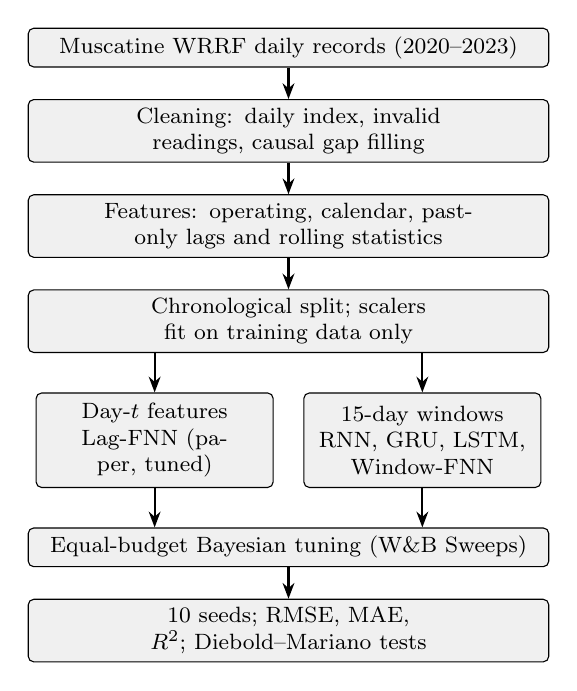
\begin{tikzpicture}[
  font=\footnotesize,
  box/.style={draw, rounded corners=2pt, align=center, inner sep=3pt, fill=black!6},
  wide/.style={box, text width=64mm},
  half/.style={box, text width=28mm, minimum height=12mm},
  arr/.style={-{Stealth[length=2mm]}, thick},
  node distance=4mm]
\node[wide] (data) {Muscatine WRRF daily records (2020--2023)};
\node[wide, below=of data] (clean) {Cleaning: daily index, invalid readings, causal gap filling};
\node[wide, below=of clean] (feat) {Features: operating, calendar, past-only lags and rolling statistics};
\node[wide, below=of feat] (split) {Chronological split; scalers fit on training data only};
\node[half, anchor=north] (fnn) at ($(split.south)+(-17mm,-5mm)$) {Day-$t$ features\\Lag-FNN (paper, tuned)};
\node[half, anchor=north] (rnn) at ($(split.south)+(17mm,-5mm)$) {15-day windows\\RNN, GRU, LSTM, Window-FNN};
\node[wide, anchor=north] (tune) at ($(rnn.south -| split.south)+(0,-5mm)$) {Equal-budget Bayesian tuning (W\&B Sweeps)};
\node[wide, below=of tune] (eval) {10 seeds; RMSE, MAE, $R^2$; Diebold--Mariano tests};
\draw[arr] (data) -- (clean);
\draw[arr] (clean) -- (feat);
\draw[arr] (feat) -- (split);
\draw[arr] (split.south -| fnn.north) -- (fnn.north);
\draw[arr] (split.south -| rnn.north) -- (rnn.north);
\draw[arr] (fnn.south) -- (tune.north -| fnn.south);
\draw[arr] (rnn.south) -- (tune.north -| rnn.south);
\draw[arr] (tune) -- (eval);
\end{tikzpicture}
\caption{Pipeline of the study. Both model families receive the same days, features and tuning budget.}
\label{fig:arch}
\end{figure}

\subsection{Features}\label{sec:features}
Following \cite{long2026}, each day has $F=35$ features: the 21 operating variables; the
month and day of the year encoded as sine and cosine pairs; the target lagged by 1, 2, 7 and 15
days; and rolling means and standard deviations of the target over 5, 10 and 15 days. The
lagged and rolling features are computed from days before $t$ only, so the label of day $t$
never enters its own inputs. We drop the year number used in \cite{long2026}: with fewer than
two training years it could only extrapolate. The published FNN keeps its min--max scaling to
$[0,1]$; all other models use z-score scaling. Both scalers are fit on the training period only.

\subsection{Models}
\emph{Persistence} predicts that today equals yesterday, $\hat{y}_t=y_{t-1}$; a useful model
must beat it.

\emph{Lag-FNN (base paper).} The 128--64--1 ReLU network of \cite{long2026} on $\mathbf{x}_t$,
trained with Adam at learning rate $10^{-3}$ and batch size 32, exactly as published and not
tuned (12,929 parameters).

\emph{Lag-FNN (tuned).} The same architecture family with depth, width, dropout, learning rate,
weight decay and batch size tuned with the same budget as the recurrent models. Beating only an
untuned baseline would not show that recurrence helps.

\emph{Recurrent models.} An encoder reads the $L$-day window and its last hidden state
$\mathbf{h}_t$ feeds a linear output, $\hat{y}_t=\mathbf{w}^\top\mathbf{h}_t+b$. The vanilla
RNN \cite{elman1990} updates
\begin{equation}
\mathbf{h}_\tau=\tanh\left(\mathbf{W}\mathbf{x}_\tau+\mathbf{U}\mathbf{h}_{\tau-1}+\mathbf{b}\right).
\end{equation}
The GRU \cite{cho2014} adds a reset gate $\mathbf{r}_\tau$ and an update gate $\mathbf{z}_\tau$,
\begin{align}
\mathbf{r}_\tau&=\sigma(\mathbf{W}_r\mathbf{x}_\tau+\mathbf{U}_r\mathbf{h}_{\tau-1}+\mathbf{b}_r),\\
\mathbf{z}_\tau&=\sigma(\mathbf{W}_z\mathbf{x}_\tau+\mathbf{U}_z\mathbf{h}_{\tau-1}+\mathbf{b}_z),\\
\tilde{\mathbf{h}}_\tau&=\tanh\left(\mathbf{W}_h\mathbf{x}_\tau+\mathbf{r}_\tau\odot(\mathbf{U}_h\mathbf{h}_{\tau-1})+\mathbf{b}_h\right),\\
\mathbf{h}_\tau&=(1-\mathbf{z}_\tau)\odot\tilde{\mathbf{h}}_\tau+\mathbf{z}_\tau\odot\mathbf{h}_{\tau-1}.
\end{align}
The LSTM \cite{hochreiter1997} keeps a cell state $\mathbf{c}_\tau$ controlled by input,
forget and output gates $\mathbf{i}_\tau,\mathbf{f}_\tau,\mathbf{o}_\tau$ (each a sigmoid of
$\mathbf{x}_\tau$ and $\mathbf{h}_{\tau-1}$),
\begin{align}
\mathbf{c}_\tau&=\mathbf{f}_\tau\odot\mathbf{c}_{\tau-1}+\mathbf{i}_\tau\odot\tanh(\mathbf{W}_c\mathbf{x}_\tau+\mathbf{U}_c\mathbf{h}_{\tau-1}+\mathbf{b}_c),\\
\mathbf{h}_\tau&=\mathbf{o}_\tau\odot\tanh(\mathbf{c}_\tau).
\end{align}
Each window step contains all 35 features, so the recurrent models see the same information
as the FNN on day $t$, plus the earlier days of the window.

\emph{Window-FNN (ablation).} An FNN on the flattened $L\times F$ window. It sees exactly the
inputs of the recurrent models but has no recurrence, so comparing them shows whether a gain
comes from recurrence or simply from a longer input.

\subsection{Training}
All neural models share one training loop in PyTorch \cite{paszke2019}: Adam
\cite{kingma2015} on the mean squared error of the scaled target, mini-batches, gradient-norm
clipping at 1.0 \cite{pascanu2013}, and up to 1,000 epochs with early stopping after 60 epochs
without improvement in validation RMSE. The weights of the best validation epoch are restored.

\subsection{Equal-budget tuning}
Hyper-parameters are tuned by Bayesian optimisation \cite{snoek2012} with Weights \& Biases
Sweeps \cite{biewald2020}, minimising validation RMSE. Every tuned model (tuned FNN,
Window-FNN, RNN, GRU, LSTM) receives the same budget of 40 sweep runs, each trained with seed~0
on the same training and validation days. The shared search space is given in
Table~\ref{tab:hp}. The window length is fixed at $L=15$ and not tuned.

\begin{table}[!t]
\centering
\caption{Hyper-parameter search space (40 runs per model)}
\label{tab:hp}
\begin{tabular}{@{}lll@{}}
\toprule
Hyper-parameter & Range & Models \\
\midrule
Learning rate & $10^{-4}$--$10^{-2}$ (log) & all \\
Weight decay & $10^{-7}$--$10^{-2}$ (log) & all \\
Batch size & \{16, 32, 64, 128\} & all \\
Dropout & 0--0.4 & all \\
Hidden layers & 1--3 & FNNs \\
First-layer width & \{32, 64, 128, 256\} & FNNs \\
Recurrent layers & 1--2 & RNN, GRU, LSTM \\
Hidden size & \{16, 32, 64, 128\} & RNN, GRU, LSTM \\
\bottomrule
\end{tabular}
\end{table}

\subsection{Evaluation}
Each model is retrained with its best hyper-parameters under ten random seeds and scored on
the test year. We report the metrics of \cite{long2026}, root mean squared error (RMSE), the
coefficient of determination $R^2$ and the share of days predicted within $\pm10\,\%$
(Acc$_{\pm10\%}$), together with the mean absolute error (MAE), as mean $\pm$ standard
deviation over seeds.

To test whether model A is more accurate than model B we apply the Diebold--Mariano (DM) test
\cite{diebold1995} to the seed-averaged predictions. With the loss differential
$d_t=(\hat{y}^A_t-y_t)^2-(\hat{y}^B_t-y_t)^2$ over the $n=365$ test days,
\begin{equation}
\mathrm{DM}=\frac{\bar{d}}{\sqrt{\hat{\sigma}^2/n}},\qquad
\hat{\sigma}^2=\hat{\gamma}_0+2\sum_{k=1}^{K}\left(1-\frac{k}{K+1}\right)\hat{\gamma}_k,
\end{equation}
where $\hat{\gamma}_k$ is the lag-$k$ autocovariance of $d_t$. Daily loss differentials are
autocorrelated, so we use this Newey--West (HAC) variance with the bandwidth
$K=\lfloor4(n/100)^{2/9}\rfloor=5$ \cite{newey1994} instead of the lag-0 variance, which would
give p-values that are too small. The statistic is compared with a $t_{n-1}$ distribution
\cite{harvey1997}; we report the one-sided p-value for ``A is more accurate than B'' and call a
difference significant at $p<0.05$.

% ---------------------------------------------------------------------------------------------
\section{Results}\label{sec:results}

\subsection{Accuracy on the test year}
Table~\ref{tab:results} lists the test scores. \tbd{Describe the ranking: which model has the
lowest RMSE and highest $R^2$, by how much it improves on the published FNN and on the tuned
FNN, and how all models compare with persistence.}

\IfFileExists{results/results_table.tex}{\input{results/results_table.tex}}{%
\begin{table}[!t]
\centering
\caption{Test results, biogas (ft$^3$/min), mean$\pm$std over 10 seeds}
\label{tab:results}
\begin{tabular}{@{}lcccc@{}}
\toprule
Model & RMSE$\downarrow$ & MAE$\downarrow$ & $R^2\uparrow$ & Acc$_{\pm10\%}\uparrow$ \\
\midrule
Persistence & \tbd{} & \tbd{} & \tbd{} & \tbd{} \\
Lag-FNN (base paper) & \tbd{} & \tbd{} & \tbd{} & \tbd{} \\
Lag-FNN (tuned) & \tbd{} & \tbd{} & \tbd{} & \tbd{} \\
Window-FNN & \tbd{} & \tbd{} & \tbd{} & \tbd{} \\
RNN & \tbd{} & \tbd{} & \tbd{} & \tbd{} \\
GRU & \tbd{} & \tbd{} & \tbd{} & \tbd{} \\
LSTM & \tbd{} & \tbd{} & \tbd{} & \tbd{} \\
\bottomrule
\end{tabular}
\end{table}}

\subsection{Statistical significance}
Table~\ref{tab:dm} gives the DM tests of each window model against both FNN baselines (from
\texttt{significance.csv}). \tbd{State which comparisons are significant at $p<0.05$ and which
are not. Do not claim a win where $p\ge0.05$.}

\begin{table}[!t]
\centering
\caption{One-sided Diebold--Mariano p-values (HAC), H$_1$: row model more accurate than column model}
\label{tab:dm}
\begin{tabular}{@{}lcc@{}}
\toprule
Model & vs.\ Lag-FNN (paper) & vs.\ Lag-FNN (tuned) \\
\midrule
RNN & \tbd{} & \tbd{} \\
GRU & \tbd{} & \tbd{} \\
LSTM & \tbd{} & \tbd{} \\
Window-FNN & \tbd{} & \tbd{} \\
\bottomrule
\end{tabular}
\end{table}

\subsection{Predictions over the test year}
Fig.~\ref{fig:pred} compares measured and predicted biogas over the test year.
\tbd{Describe where the models follow the measurements and where they miss, e.g.\ sudden
drops or peaks.}

\begin{figure}[!t]
\centering
\IfFileExists{results/test_Biogas.pdf}{%
\includegraphics[width=\columnwidth]{results/test_Biogas.pdf}}{%
\fbox{\parbox[c][35mm][c]{0.9\columnwidth}{\centering\tbd{results/test\_Biogas.pdf}}}}
\caption{Measured and predicted daily biogas over the test year (seed-averaged predictions).}
\label{fig:pred}
\end{figure}

% ---------------------------------------------------------------------------------------------
\section{Discussion}\label{sec:discussion}

\subsection{Recurrence or a longer window?}
The Window-FNN receives the same 15-day input as the recurrent models.
\tbd{If the recurrent models beat the Window-FNN: the gain comes from how they process the
sequence, not just from seeing more days. If not: say that the longer input explains most of
the gain.}

\subsection{Gated and ungated recurrent cells}
\tbd{Explain the GRU/LSTM result. Possible reasons if the plain RNN does as well or better: with
only 467 training days and a 15-day window, the extra gate parameters of GRU and LSTM add
variance without a long-range dependency to exploit, in line with \cite{chung2014}, who found
no consistent winner among gated cells.}

\subsection{Relation to the base paper}
The $R^2$ of 0.67 reported in \cite{long2026} was obtained on a different plant, feedstock
and test year, so it is context only and cannot be compared directly with our scores. Our claim
is a within-dataset comparison: on the same days, features and budget, \tbd{finding}.

\subsection{Limitations}
The study uses one plant and one test year. The public data has no methane or H$_2$S
measurements, so only biogas flow is predicted. The inputs of day $t$ include that day's
operating measurements, so the task is same-day estimation from operating data and past
production rather than a forecast several days ahead. Only one window length ($L=15$) is
reported in the main results. \tbd{Add the $L=30$ ablation here if it is run.}

% ---------------------------------------------------------------------------------------------
\section{Conclusion}

We compared vanilla RNN, GRU and LSTM networks with the lag-feature FNN of a recent
commercial-digester study on the public daily data of a full-scale co-digestion plant. All
models had the same chronological split, features and tuning budget and were evaluated over
ten seeds with autocorrelation-robust significance tests. \tbd{Main result in one or two
sentences.} Future work will extend the task to multi-day-ahead forecasts, data from more
plants, and gas-quality targets such as methane and H$_2$S, and will study how predictions can
support feeding decisions.

\section*{Data and Code Availability}
The Muscatine data is public \cite{muscatinedata} under the ODC-By 1.0 licence. Our code, the
split definitions and the tuning logs are available at \tbd{repository URL}.

\section*{Acknowledgment}
We thank H.~W.~Schroer and C.~L.~Just for releasing the Muscatine operating data.

\bibliographystyle{IEEEtran}
\bibliography{refs}

\end{document}
